\chapter{Conception Logicielle}

Après avoir défini la persistance, nous avons structuré l'application en deux couches principales : le backend Node.js, qui fournit l'API REST, et le frontend Angular, qui orchestre l'interface et la manipulation des données côté client.

\section{Schéma d'architecture applicative}
Le schéma ci-dessous illustre l'architecture applicative de l'application Angular et les principaux services métiers. Il montre comment les composants, les modèles et les services collaborent pour gérer les locaux, le personnel, le matériel et les prises. Bien que présenté sous forme de diagramme synthétique, il ne s'agit pas d'un diagramme de classes UML strict mais d'une représentation opérationnelle des composants et de leurs interactions.

\begin{figure}[h]
    \centering
    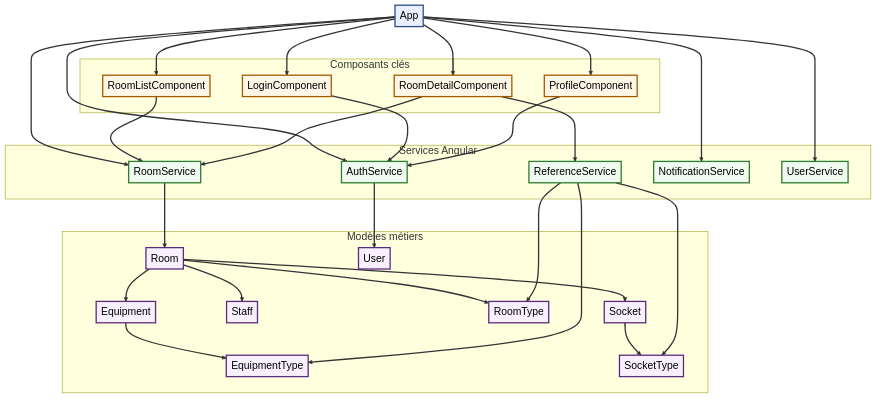
\includegraphics[width=\linewidth,keepaspectratio]{img/diagramme_classes_uml.png}
    \caption{Schéma d'architecture applicative - Angular}
    \label{fig:uml_logiciel}
\end{figure}

\newpage

\section{Principes de développement}
La conception logicielle privilégie une séparation claire des responsabilités entre :
\begin{itemize}
    \item \textbf{Modèles} : Les classes \texttt{Room}, \texttt{Equipment}, \texttt{Staff}, \texttt{RoomType}, \texttt{EquipmentType} et \texttt{SocketType} définissent les entités manipulées par le client.
    \item \textbf{Services} : Les services Angular (\texttt{RoomService}, \texttt{AuthService}, \texttt{ReferenceService}, \texttt{EquipmentService}, \texttt{StaffService}, \texttt{SocketService}) encapsulent l'accès aux API et la logique de synchronisation des données.
    \item \textbf{Composants} : Les composants gèrent l'affichage et l'interaction utilisateur : liste des salles, détail d'une salle, gestion des types, connexion, etc.
\end{itemize}

Cette architecture améliore la maintenabilité du projet. Le backend reste léger et modulaire, tandis qu'Angular assure un rendu dynamique et une expérience utilisateur fluide.

\subsection{Gestion d'état et réactivité (RxJS)}
Au-delà de la structuration classique, nous avons implémenté une gestion d'état réactive basée sur RxJS. L'utilisation de BehaviorSubject dans nos services, notamment RoomService et FloorService, agit comme une source de vérité unique. Lorsqu'une donnée est modifiée par un composant, le flux de données propage instantanément la mise à jour à tous les autres composants abonnés. Ce patron de conception avancé permet une interface fluide sans rechargement de page, garantissant que la vue 2D, 3D et les listes soient toujours cohérentes avec l'état actuel de la base de données.

\section{Sécurité et gestion des mots de passe}
Le backend gère l'authentification des utilisateurs et le stockage sécurisé des mots de passe. Concrètement, les mots de passe sont hachés côté serveur (fonction `hashPassword` dans `back/config/auth.js`) à l'aide d'un dérivé sécurisé (scrypt) avant d'être persistés en base. La vérification (`verifyPassword`) compare de façon sécurisée le mot de passe fourni avec le haché stocké. Par mesure de sécurité, il est recommandé de changer le mot de passe administrateur par défaut fourni dans les scripts d'initialisation dès le premier déploiement, et d'utiliser des secrets/variables d'environnement pour les identifiants en production.
